$z = f(x, y) = x^3 - 3xy^2$ \\
Gradient of f(x, y):
$$\vec{\nabla} f = \begin{bmatrix}
	\frac{\partial f}{\partial x} \\[6pt]
	\frac{\partial f}{\partial y}
\end{bmatrix} $$
$$\vec{\nabla} f = \begin{bmatrix}
	3x^2 - 3y^2 \\
	-6xy
\end{bmatrix} $$
Two linear equations with two unknowns.
$$	3x^2 - 3y^2 =  0 $$
$$-6xy = 0$$
Answers is $x = 0$ and $y = 0$.


Hessian matrix:
$$H = \frac{\partial^2 f}{\partial \vec{X}^2} = \begin{bmatrix}
	\frac{\partial^2 f}{\partial x^2} & \frac{\partial^2 f}{\partial xy} \\[6pt]
	\frac{\partial^2 f}{\partial yx}  & \frac{\partial f}{\partial y^2}
\end{bmatrix} $$
$$H = \begin{bmatrix}
	6x & -6y \\
   -6y & -6x
\end{bmatrix}$$



In $x = 0$ and $y = 0$ Hessian matrix in :
$$H = \begin{bmatrix}
	0 & 0 \\
	0 & 0
\end{bmatrix}$$
so this point is saddle point.
\begin{figure}[H]
	\caption{3D figure of function}
	\centering
	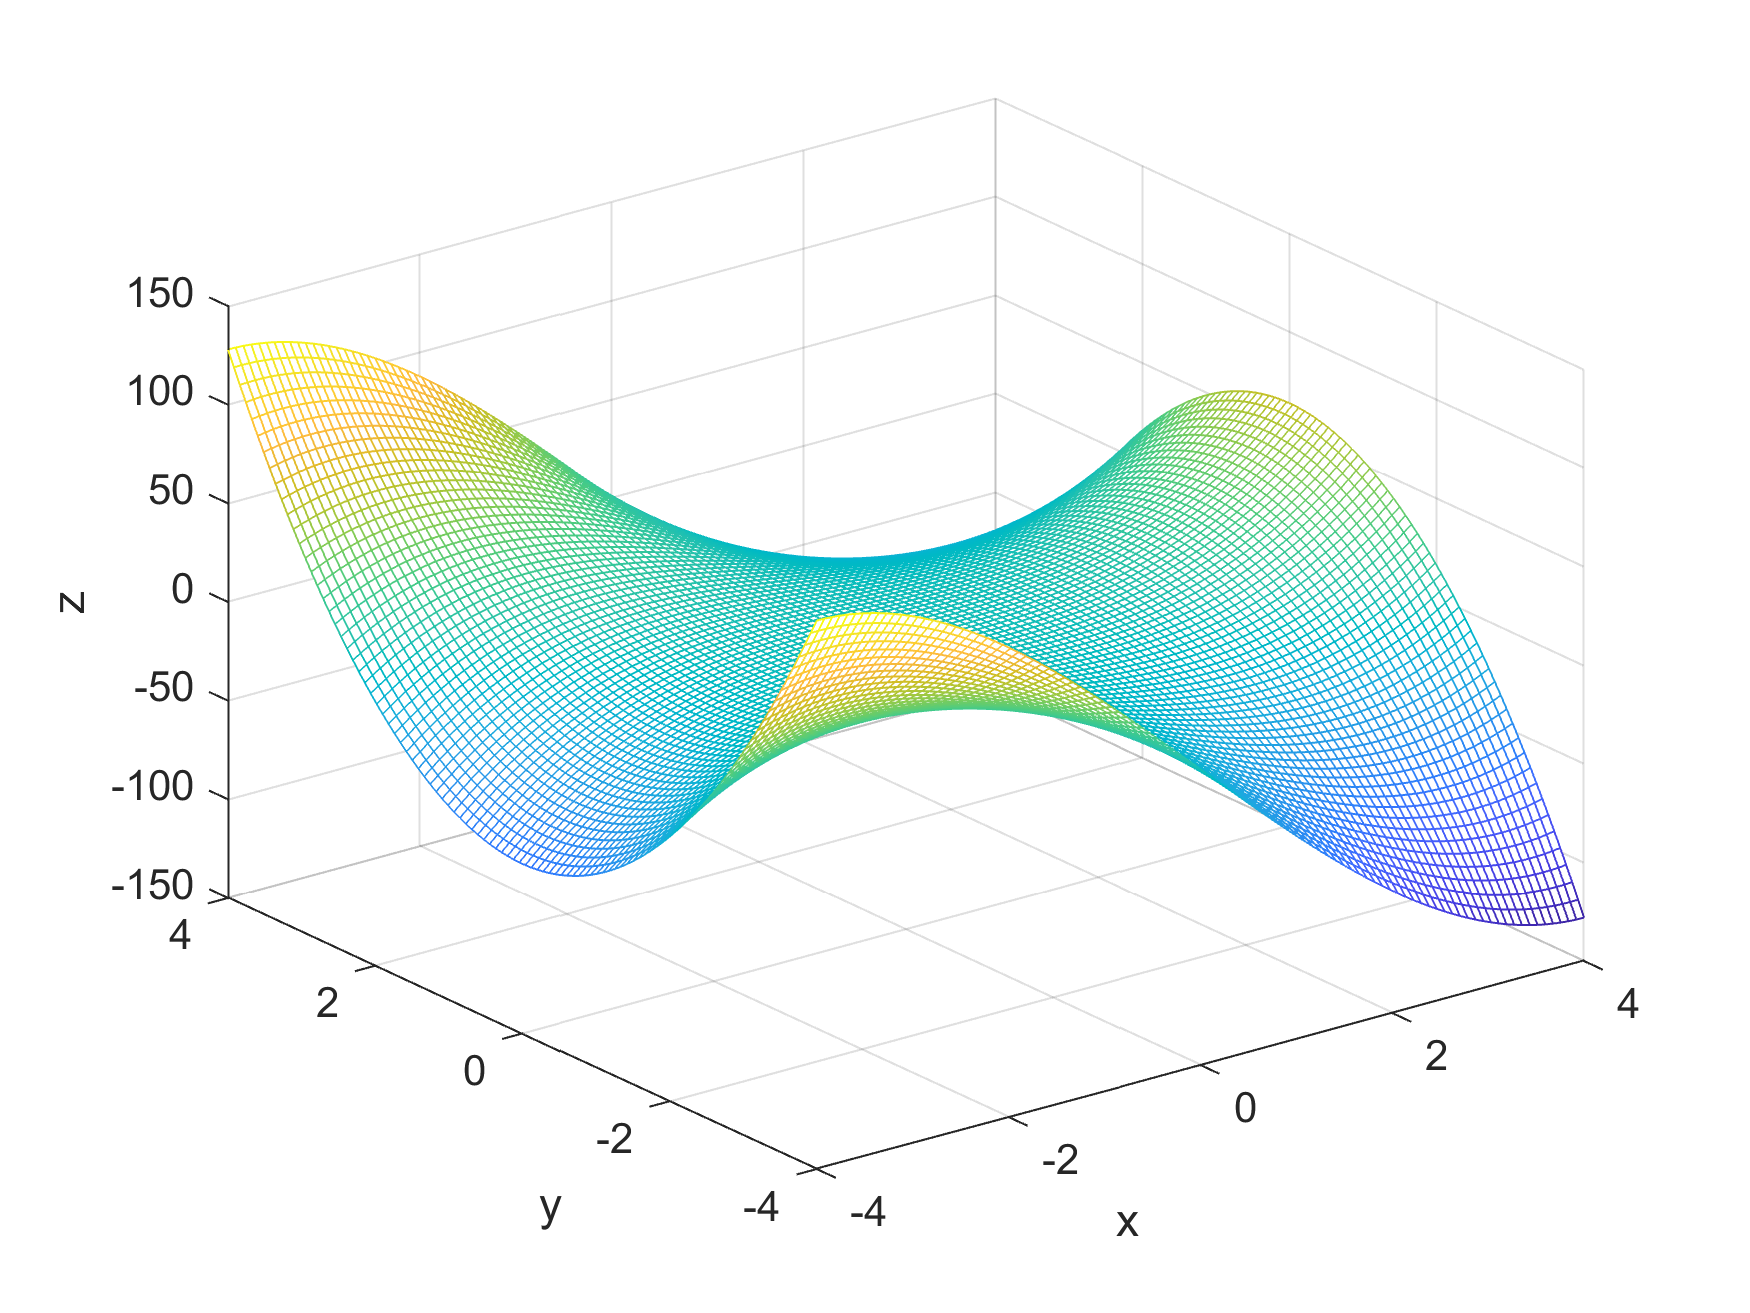
\includegraphics[width=12cm]{Q1/figures/3DplotQ1b.png}
\end{figure}

\begin{figure}[H]
	\caption{3D figure of function with Points}
	\centering
	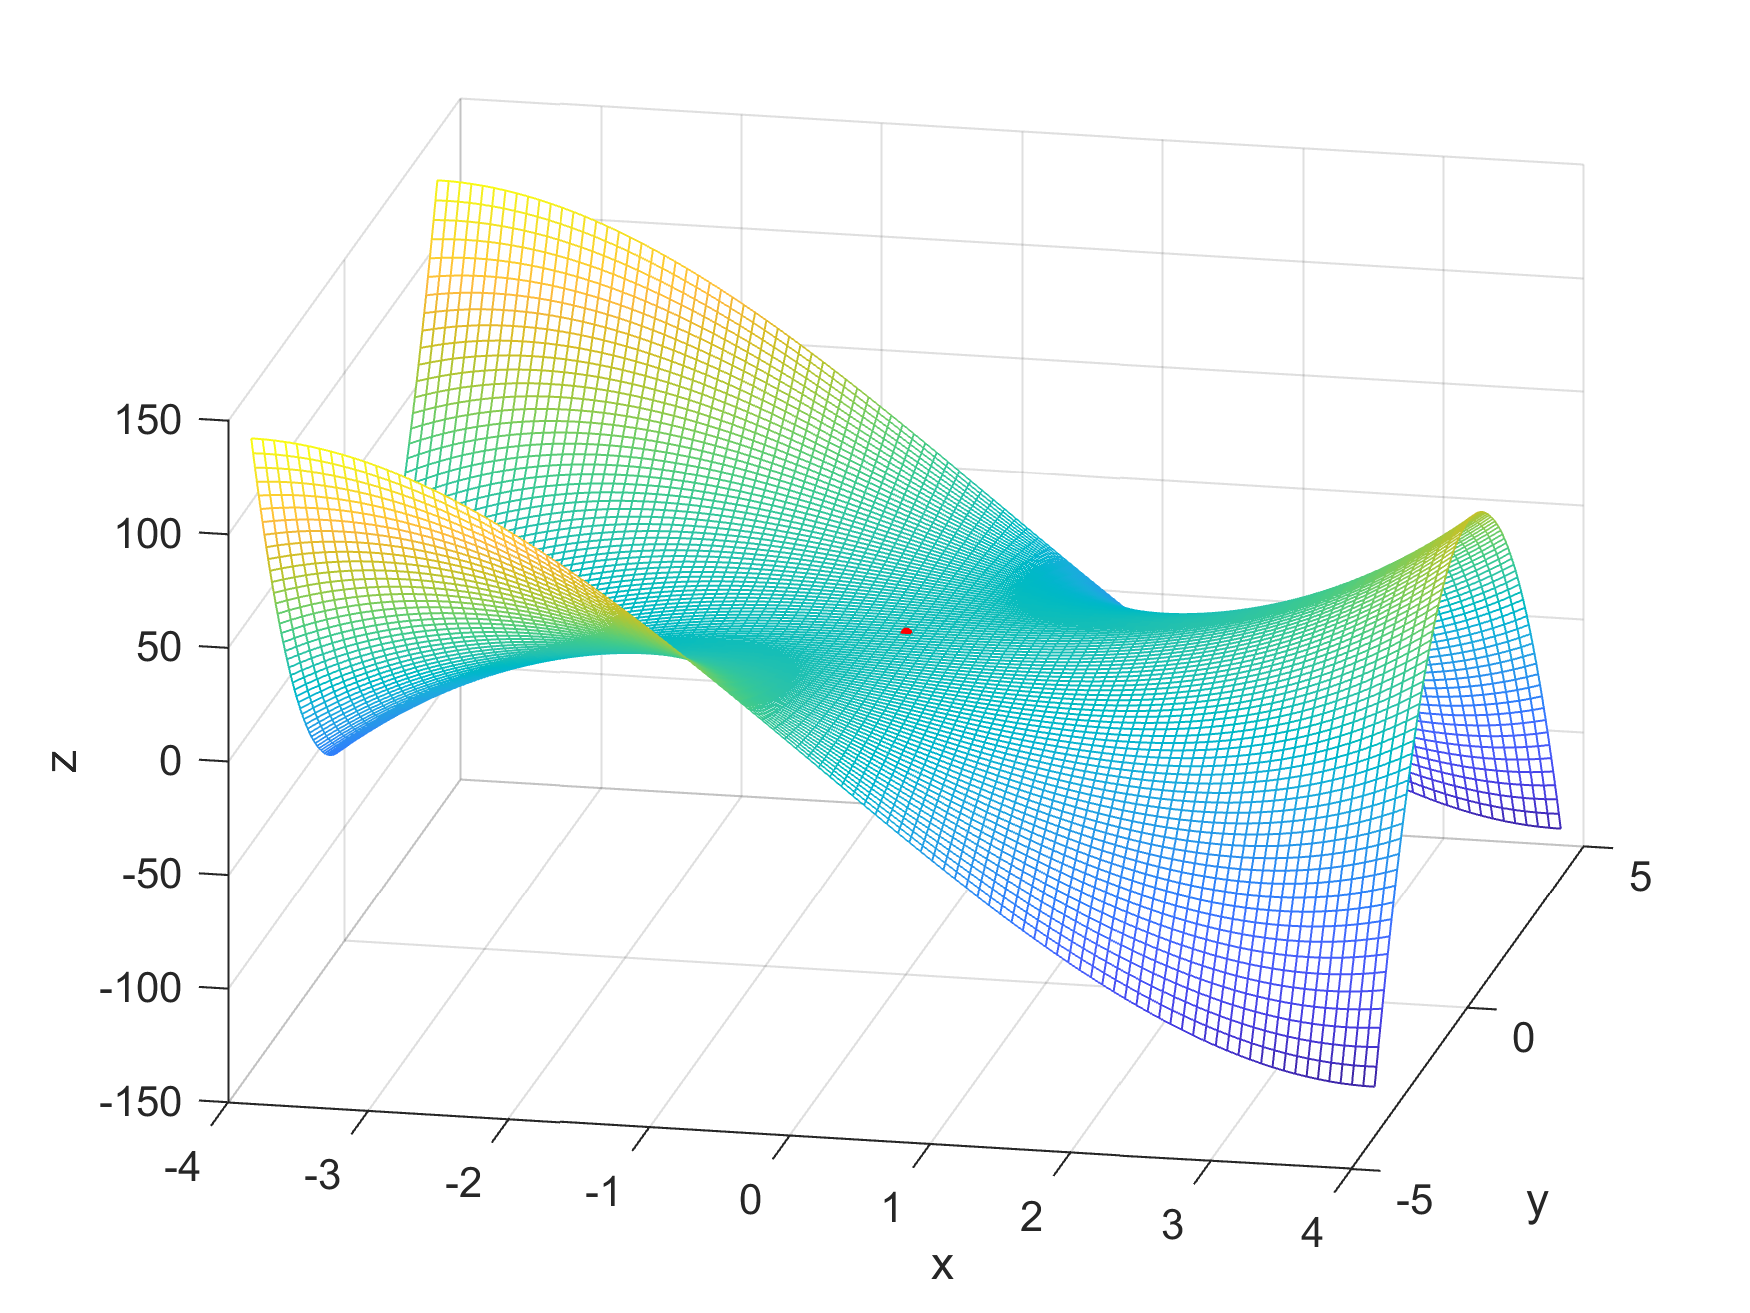
\includegraphics[width=12cm]{Q1/figures/3DplotWithPointsTashihQ1b.png}
\end{figure}

\begin{figure}[H]
	\caption{Contour figure of function}
	\centering
	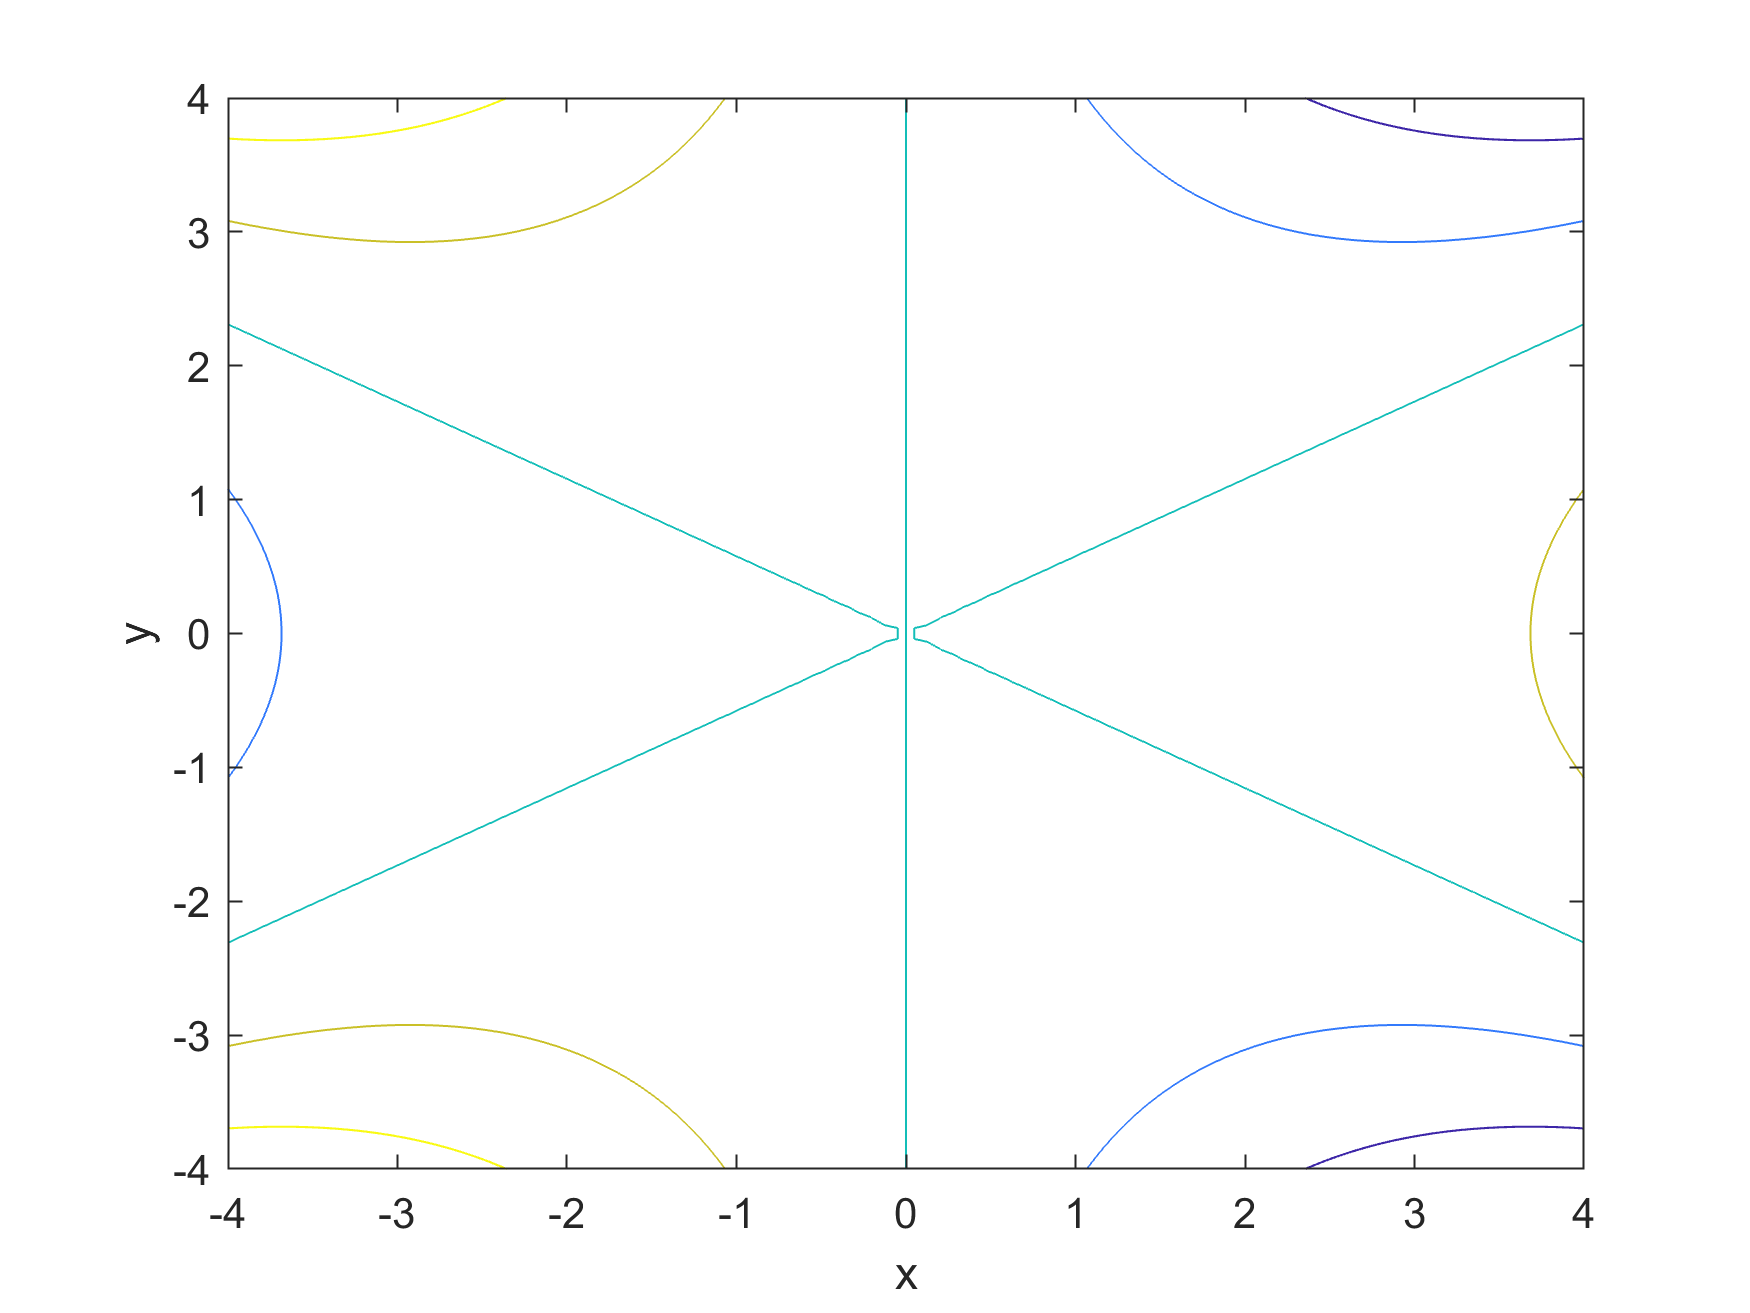
\includegraphics[width=12cm]{Q1/figures/ContourQ1b.png}
\end{figure}
\begin{figure}[H]
	\caption{Contour figure of function with Points}
	\centering
	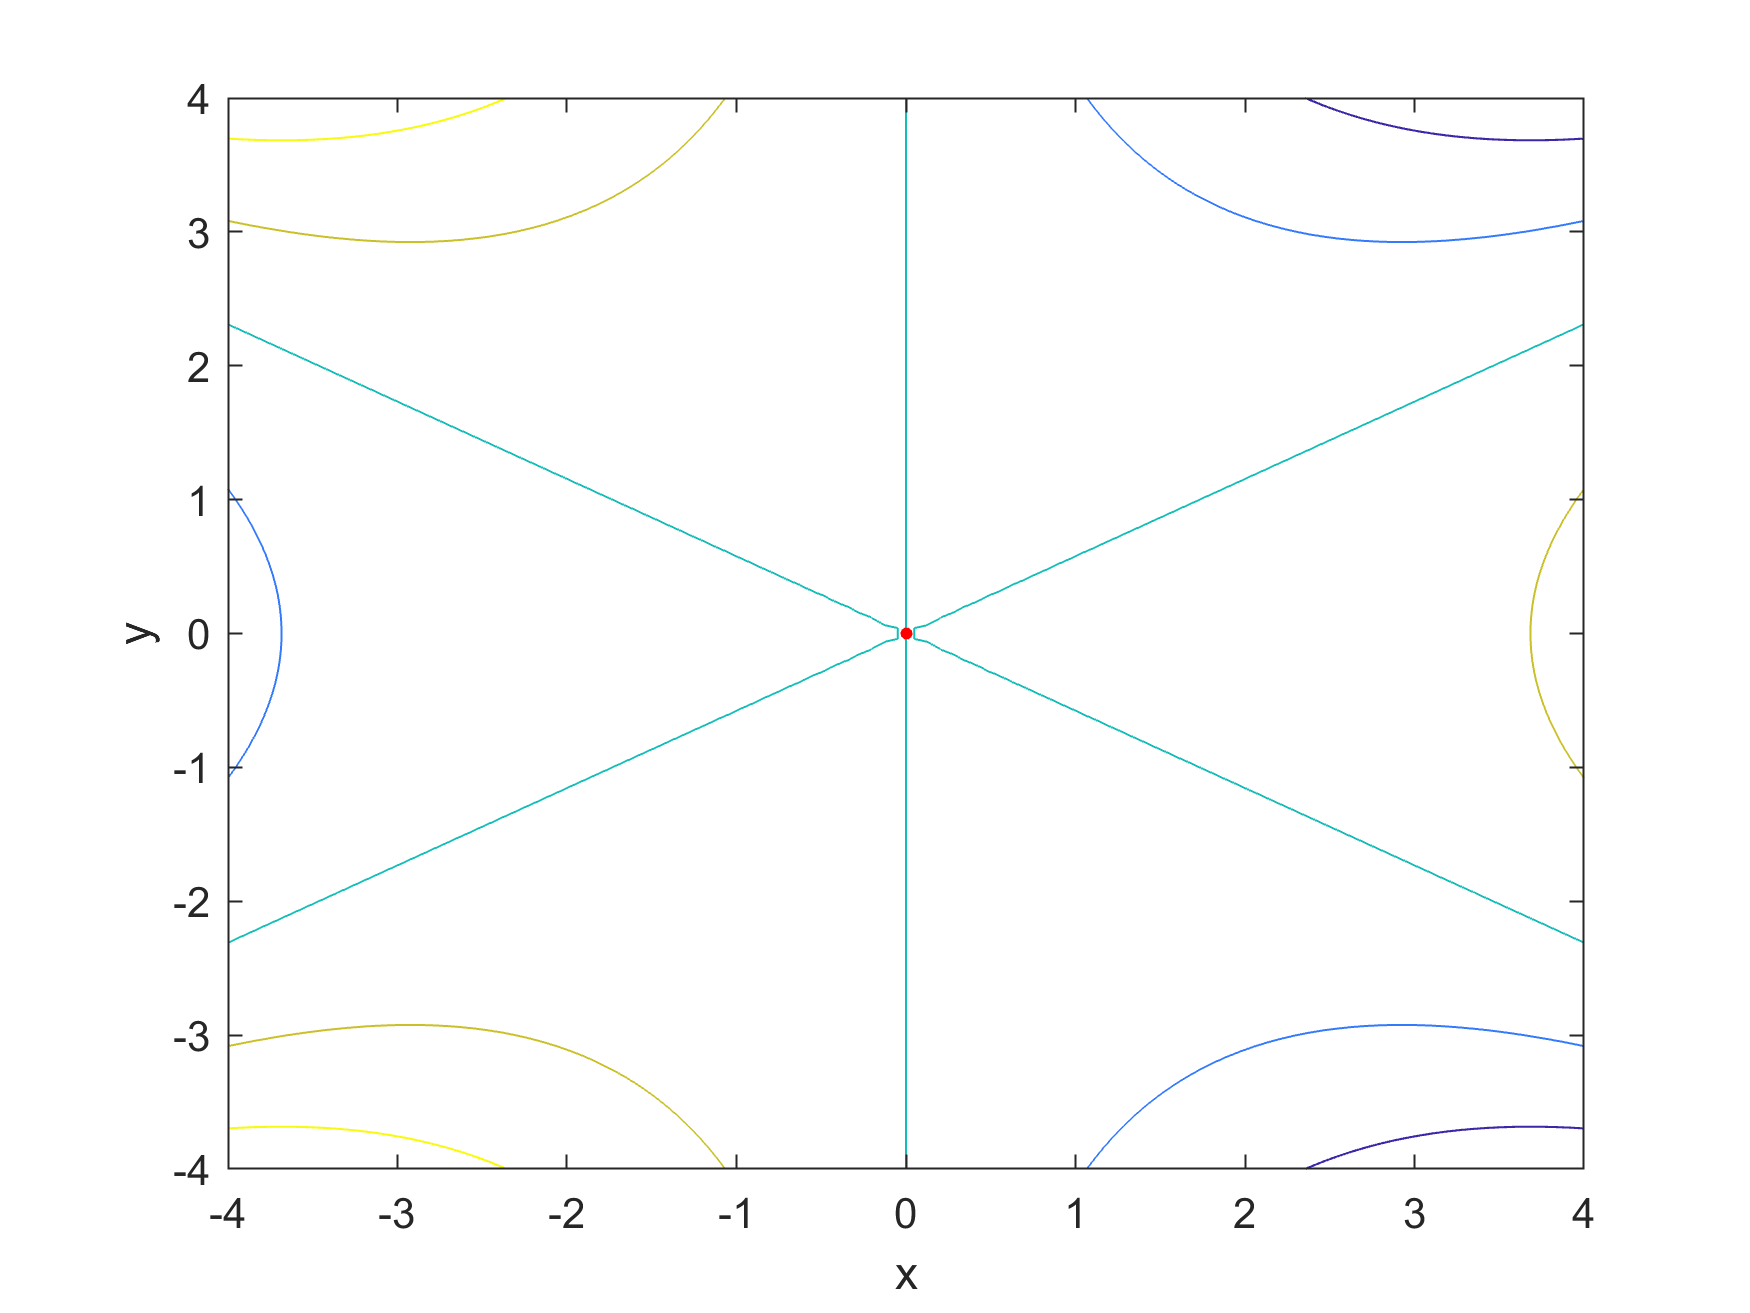
\includegraphics[width=12cm]{Q1/figures/ContourWithPointsQ1b.png}
\end{figure}
